\begin{frame}
\frametitle{Introduction}
	\begin{figure}
		\centering
		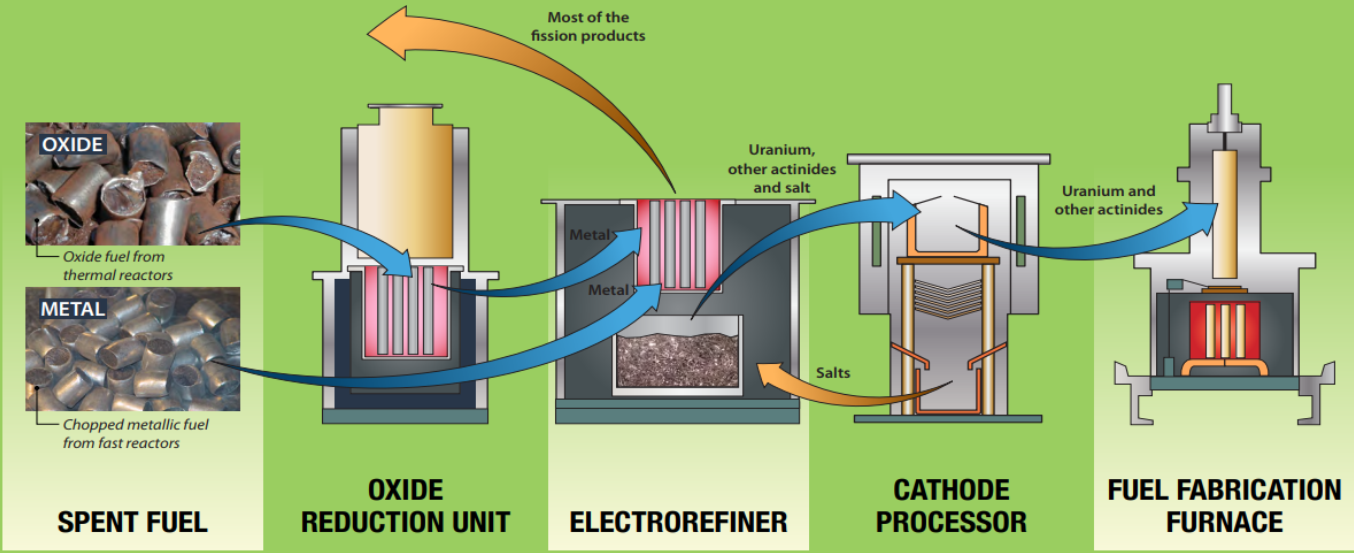
\includegraphics[width=\linewidth]{pyro-background.png}
		\caption{Argonne demonstration of a basic pyro plant \cite{williamson_pyroprocessing_nodate}.}
		\label{fig:pyro}
	\end{figure}
\end{frame}

\begin{frame}
\frametitle{Motivation/Goals}
\textbf{Motivation}
\begin{itemize}
	\item Safeguard by design
	\item Model diversion inside facilities
	\item transition from LWR to SFR
\end{itemize}
\textbf{Goals}
\begin{itemize}
	\item Detect diversion using signatures and observables.
	\item Optimum detector and inspection locations in pyroprocessing
	\item Characterize detection sensitivities and false positive rates
\end{itemize}
\end{frame}


\begin{frame}
\frametitle{Inspiration}
\begin{figure}
\centering

\includegraphics[width=0.9\linewidth]{borrelli-citation.png}
\end{figure}
\end{frame}